\documentclass[12pt,letter]{article}

\usepackage{amsmath}
\usepackage{hyperref}
\usepackage{graphicx}
\usepackage{verbatim}
\usepackage{xcolor}
\usepackage{listings}
\lstset{%
    basicstyle=\scriptsize\ttfamily, %
    language=Matlab, %
    keywordstyle=\color{blue},%
    commentstyle=\color{green!50!black},%
    numberstyle=\color{gray},%
    stringstyle=\color{magenta!70!blue},%
    deletekeywords={type},%
    otherkeywords={xlim,ylim,ones},%
    numbers=left,%
    showstringspaces=false,%
}

\usepackage{tikz}

\tikzstyle{block}=[rectangle,draw=black,thick,minimum size=1.2cm]
\tikzstyle{signal}=[rectangle,text width=1.0cm]
\tikzstyle{junction}=[circle,fill=black,draw=black,inner sep=0,minimum size=1.0mm]
\tikzstyle{operator}=[circle,draw=black,thick,inner sep=2pt]

\newcommand{\ts}[1]{\textsuperscript{#1}}
\newcommand{\rpref}[1]{\ref{#1} on page \pageref{#1}}

\title{ECE480A3 Project Final Report: \\ Diagnosis of Cardiac Arrhythmias from 
Electrocardiography Data}
\author{Robby Stokoe}
\date{\today}

\begin{document}
\maketitle

\begin{abstract}
    The diagnosis of cardiac arrhythmias can be a tedious process when done by
    hand and could benefit greatly from computer automation.  To this end, an
    algorithm was developed to distinguish between normal heart beats and
    abnormal arrhythmic beats in an ECG waveform.  First an algorithm was
    developed to find the location of QRS complexes in the ECG waveform.
    Principal component analysis was performed using the area around the QRS
    complex.  20 of the resulting principal components were used to train a
    simple linear classifier to distinguish between normal and abnormal beats.
    The classification performed reasonably well with a sensitivity of 85.4\%
    and specificity of 91.7\%. More- sophisticated signal processing and
    classification techniques could be applied to improve these numbers, but the
    algorithm is good starting point.  
\end{abstract}

\section{Introduction} 
Cardiac arrhythmias are a relatively common set of diseases, affecting 3.4\% of
people in the US \cite{cdc95}.  Diagnosis is done by eye from an ECG trace which
can be tedious.  A common diagnostic technique is to record ECG data from a
patient constantly as they go about normal activity.  This results in a very
long recording which may contain only a few abnormal beats.  An algorithm-driven
diagnosis could potentially eliminate this tedium and also the possibility of
human error if the algorithm is robust enough.  Such an algorithm could be used
in AEDs, pacemakers, or EEG machines.  Even if the algorithm is not as robust as
human diagnosis, it could still assist diagnosis by flagging potentially
abnormal beats for further analysis, allowing a trained cardiologist to quickly
zero-in on the relevant beats.  This project attempts to develop such an
algorithm using signal processing and classification techniques.  

\section{Data}
The data used to develop the signal processing algorithm and train the
classifier were obtained from the MIT-BIH Arrhythmia Database which is available
on \url{physionet.org}.  The data and techniques used to obtain it are described
as follows: 
\begin{quotation}
     The MIT-BIH Arrhythmia Database contains 48 half-hour excerpts of
     two-channel ambulatory ECG recordings, obtained from 47 subjects studied by
     the BIH Arrhythmia Laboratory between 1975 and 1979. Twenty-three
     recordings were chosen at random from a set of 4000 24-hour ambulatory ECG
     recordings collected from a mixed population of inpatients (about 60\%) and
     outpatients (about 40\%) at Boston's Beth Israel Hospital; the remaining 25
     recordings were selected from the same set to include less common but
     clinically significant arrhythmias that would not be well-represented in a
     small random sample.

     The recordings were digitized at 360 samples per second per channel with
     11-bit resolution over a 10 mV range. Two or more cardiologists
     independently annotated each record; disagreements were resolved to obtain
     the computer-readable reference annotations for each beat (approximately
     110,000 annotations in all) included with the database.
\end{quotation}

The data and annotations will be instrumental in training and testing the
classification algorithm.  Figure \ref{fig:raw} shows a portion of a recording
from the Database with annotations showing normal beats, an atrial premature
beat (A) and a premature ventricular contraction (V).  

\section{Algorithm}
The first step of the algorithm will be to identify the locations of QRS
complexes in the ECG.  This will be done by the Pan-Tompkins algorithm shown
schematically in Figure \ref{fig:pan}.  This algorithm works by differentiating
the signal, squaring the derivative, and then comparing the resulting squared
derivative with some threshold.  The location of the maximum absolute value of
the signal where the squared derivative is above the threshold is taken to be
the location of the R-wave in the QRS complex \cite{pan-tompkins85}

\begin{figure}[hbtp]
    \centering
    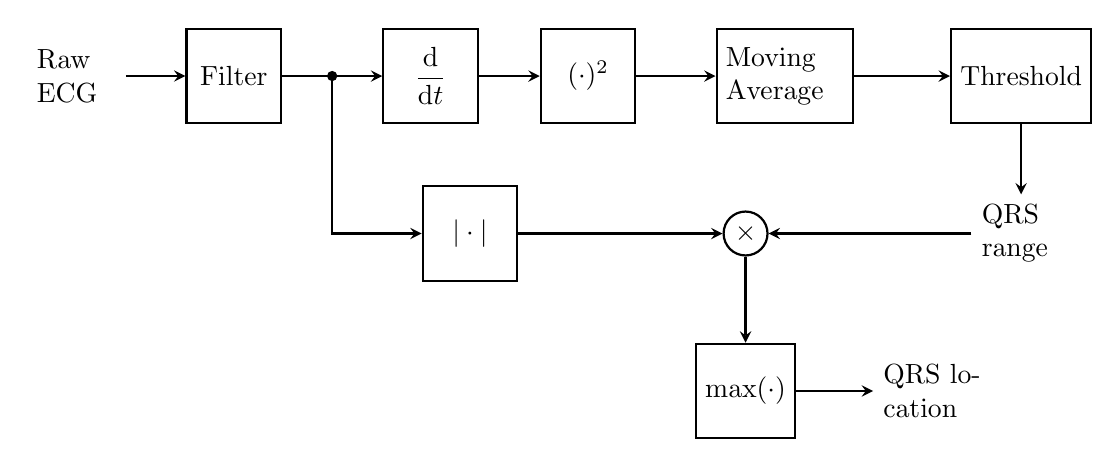
\begin{tikzpicture}[thick,>=stealth]
        \node[signal] (input) at (-6.5,0) {Raw ECG};
        \node[block] (filter) at (-4.5,0) {Filter};
        \node[block] (deriv)  at (-2,0) 
            {$\displaystyle\frac{\mathrm{d}}{\mathrm{d}t}$};
        \node[block] (square) at (0,0)  {$(\cdot)^2$};
        \node[block] (thresh) at (5.5,0) {Threshold};
        \node[signal] (range) at (5.5,-2)  {QRS range};
        \node[block,text width=1.5cm] (avg) at (2.5,0) {Moving Average};
        \node[block] (abs) at (-1.5,-2) {$|\cdot|$};
        \node[operator] (mult) at (2.0,-2) {$\times$};
        \node[block] (max) at (2.0,-4) {$\max(\cdot)$};
        \node[signal,text width=1.5cm] (location) at (4.5,-4) {QRS location};

        \draw [->] (input) -- (filter);
        \draw [->] (filter) -- node[junction] (branch) {} (deriv.west);
        \draw [->] (deriv) -- (square);
        \draw [->] (square) -- (avg);
        \draw [->] (avg) -- (thresh);
        \draw [->] (thresh) -- (range);
        \draw [->] (range) -- (mult);
        \draw [->] (mult) -- (max);
        \draw [->] (branch) |- (abs);
        \draw [->] (abs) -- (mult);
        \draw [->] (max) -- (location);
    \end{tikzpicture}
    \caption{The Pan-Tompkins Algorithm for Finding QRS Complexes}
    \label{fig:pan}
\end{figure}

Once the location of the center of the QRS complex is determined, the portion of
the signal few hundred milliseconds before and after the QRS complex is
extracted for analysis.  To train the classifier, a multitude of these signal
excerpts were gathered and sorted by normal \textit{vs.} abnormal rhythm.
Principal component analysis was performed on this entire data set to obtain a
transformation to be used for classification.  Only some of the components of
this transformation were used to simplify classification.  To obtain the best
discrimination between normal and abnormal beats, the components for which the
mean values of the normal and abnormal beats were the most significantly
different were used.  In addition to the principal components, the R-R interval
for each beat was also found and used as an additional component.  

\section{Implementation}

The algorithm was implemented in MATLAB.  All code used is included in the
appendix and available on github at
\url{https://github.com/robbystk/Arrythmias}. The first step was to download ECG
data and annotations from Physionet using the \verb`rdsamp()` and \verb`rdann()`
functions from Physionet's WFDB toolbox.  These functions were wrapped in
another function, \verb`fetch()`, to make them easier to use.  See page
\pageref{fun:fetch} for the full function.  Figure \ref{fig:raw} shows an
example of ECG data directly from physionet with beat annotations.  The
annotations do not always correspond directly with the location of the QRS
complex because they correspond to the entire beat rather than a specific
feature.  So the next step is to determine the exact location of the QRS
complexes.  

\begin{figure}[hbtp]
    \centering
    \includegraphics[height=0.44\textheight]{../figures/figures_01}
    \caption{Examples of Raw ECG Signals Showing Normal Beats (N), an Atrial
    Premature Beat (A), and Premature Ventricular Contraction (V)}
    \label{fig:raw}
\end{figure}

The first step in the Pan-Tomkins QRS-Detection algorithm is to filter the
signal.  This was done by a fourth-order Butterworth bandpass filter with
cutoffs at 1 and 50Hz, as well as a notch filter at 60Hz.  The full
implementation is shown in the \verb`filterecg()` function in section
\rpref{fun:filter}.  The effect of this filter on an ECG signal is shown in
Figure \ref{fig:filter}.  The rest of the QRS-detection algorithm was
implemented in the function \verb`findqrs()` shown in section \rpref{fun:qrs}.
Figure \ref{fig:qrs} shows an example of the signals at each stage of the
algorithm.  The QRS-detection function performed relatively well, accurately
finding the location of the QRS complex of most beats.  Occasionally it would
miss a particularly malformed beat, or find a beat were there was none,
especially if the signal was particularly noisy.  Figure \ref{fig:perf} shows a
closer look at the location of the R-wave determined by the algorithm, and an
example of some erroneously-detected beats.

\begin{figure}[hbtp]
    \centering
    \includegraphics[height=0.44\textheight]{../figures/figures_02}
    \caption{The Effect of \texttt{filterecg()} on an ECG Signal}
    \label{fig:filter}
\end{figure}

\begin{figure}[hbtp]
    \centering
    \includegraphics[height=0.42\textheight]{../figures/figures_03}
    \caption{Example Signals at the Various Stages of the Pan-Tompkins
    QRS-Detection Algorithm}
    \label{fig:qrs}
\end{figure}

\begin{figure}[hbtp]
    \centering
    \includegraphics[height=0.42\textheight]{../figures/figures_04}
    \caption{Performance of the QRS-Detection Algorithm}
    \label{fig:perf}
\end{figure}

Based on initial investigation of the data, it was decided to develop a
classifier to distinguish between normal and atrial premature beats, because
these beats deviate little from normal beats, which will give the starting point
for the entire classifier, the QRS-detection algorithm, more to work with.  

To train the classifier, a large amount of data was collected and processed (see
\verb`gather.m` in Section \rpref{scr:gather}).  Five recordings from the
MIT-BIH ECG database were chosen because they include a large number of atrial
premature beats.  These recordings were downloaded from physionet
(\verb`gather.m` lines 3--10), and processed to extract a 0.6-second excerpt
centered around the QRS complex for each normal and abnormal beat (lines
12--48).  For each recording, the locations of normal and abnormal beats were
determined from the included annotations (lines 16--20).  An equal number of
normal and abnormal beats were randomly selected (lines 21--23) and extracted
(lines 25--48).  The extraction process involved finding the QRS complex
locations with \verb`findqrs()` (lines 25--29), and extracting the signal 0.3
seconds before and after the QRS complex for both normal (lines 39--46) and
abnormal (lines 31--37) beats.  The beat excerpts were compiled into two
matrices (lines 36 and 45) for subsequent processing.  The function
\verb`crop()`, shown in Section \rpref{fun:crop}, was created to facilitate
extraction of the 0.6-second excerpts around each beat.  

The data from \verb`gather.m` were further processed and used to train a linear
classifier in \verb`train.m` shown in Section \rpref{scr:train}.  The normal and
abnormal beat data were combined into one matrix (\verb`train.m` line 10) and
normalized by subtracting the mean of each time point (lines 12--17).  Singular
value decomposition was performed on the normalized data (line 19) to find a
transformation matrix to transform the data onto an orthogonal basis of
principal components.  A visualization of the transformation matrix is shown in
Figure \ref{fig:transform} along with an example ECG waveform for reference.
Each row of the matrix produces a different principal component as a linear
combination of the value at each sample of the ECG signal.  The matrix is
arranged so that the first principal component has the highest variance across
the data.  Figure \ref{fig:var} shows the variances of the first 30 (out of 215)
principal components.  

\begin{figure}[htbp]
    \centering
    \includegraphics[height=0.42\textheight]{../figures/train_01}
    \caption{Principal Component Transformation Matrix with Reference ECG}
    \label{fig:transform}
\end{figure}

\begin{figure}[htbp]
    \centering
    \includegraphics[height=0.42\textheight]{../figures/train_02}
    \caption{Variances of the First 30 Principal Components}
    \label{fig:var}
\end{figure}

In a linear classifier, high variance of a particular measurement does not
necessarily correspond to better discrimination between two groups of data.  It
is possible for the two groups to each have a wide distribution that overlaps
almost completely with the other.  This would result in a large variance, but no
ability to categorize the data.  On the other hand, it is possible for each
group to have a narrow distribution, separated relatively little from the other
group, but significant relative to the standard deviation.  For this reason, the
components chosen to classify the data were not those with the most variance.
Instead, the mean of each component for the two groups, normal and abnormal, was
found (\verb`gather.m` lines 48--62).  The difference between these means (line
63) normalized by the variance of that particular component, was used to select
the top 20 `most-significant' components to be used for classification (lines 73
and 83).  Figure \ref{fig:diff} shows the difference in means for the first 30
Principal components (those with the largest variances).  Figure \ref{fig:sig}
shows the 20 most-significant components (those with the most significant
difference between the mean of the normal and abnormal data).  

\begin{figure}[htbp]
    \centering
    \includegraphics[height=0.42\textheight]{../figures/train_03}
    \caption{Difference in Means for First 30 Principal Components (Those with
    the Largest Variance)}
    \label{fig:diff}
\end{figure}

\begin{figure}[hbtp]
    \centering
    \includegraphics[height=0.42\textheight]{../figures/train_04}
    \caption{Difference In Means for the First 20 Most-Significant Components
    (Those with the Largest Difference In Means)}
    \label{fig:sig}
\end{figure}

The 20 most-significant components were used to train a linear classifier
(\verb`train.m` lines 91--97) using the formula $\mathbf{w} = (\mathbf{X}^\top
\mathbf{X})^+ \mathbf{X}^\top \mathbf{d}$ where $\mathbf{w}$ is a vector of
weights for each component, $\mathbf{X}$ is the matrix of data with each column
corresponding to a component and each row corresponding to a single point, and
$\mathbf{d}$ is a vector of the desired response of the classifier for each row
in $\mathbf{X}$.  In this case, $d_i = 0$ for normal beats, and 1 for abnormal
beats.  Note also that $\mathbf{A}^+$ denotes the pseudo inverse of $\mathbf{A}$
computed by MATLAB's \verb`pinv()` function.  Figure \ref{fig:classifier} shows
the first two most-significant components and the decision boundary for those
two components when every other component is equal to zero.  Note that since
this is a two-dimensional projection of 20-dimensional data, which side of the
line the a point falls on does not necessarily correspond to how it is
classified.  All 20 dimensions are necessary to classify each point.  

\begin{figure}[hbtp]
    \centering
    \includegraphics[height=0.42\textheight]{../figures/train_05}
    \caption{First Two Most-Significant Components and Cross-Section of the
    Classifier's Decision Boundary}
    \label{fig:classifier}
\end{figure}

\section{Performance} 
The classifier result was calculated (\verb`train.m` line 117) and compared to
the desired result to determine the number of true negatives, false positives,
false negatives, and true positives (lines 118--121).  These results are shown
in the confusion matrix in Figure \ref{fig:confusion}. The true positive rate
(sensitivity) and true negative rate (specificity), were also determined.  The
sensitivity was found to be $\mathrm{TPR} = \frac{\mathrm{true}
+}{\mathrm{actual} +} = 85.4\%$, and the sensitivity was found to be
$\mathrm{TNR} = \frac{\mathrm{true} -}{\mathrm{actual} -} = 91.7\%$

\begin{figure}[htbp]
    \centering
    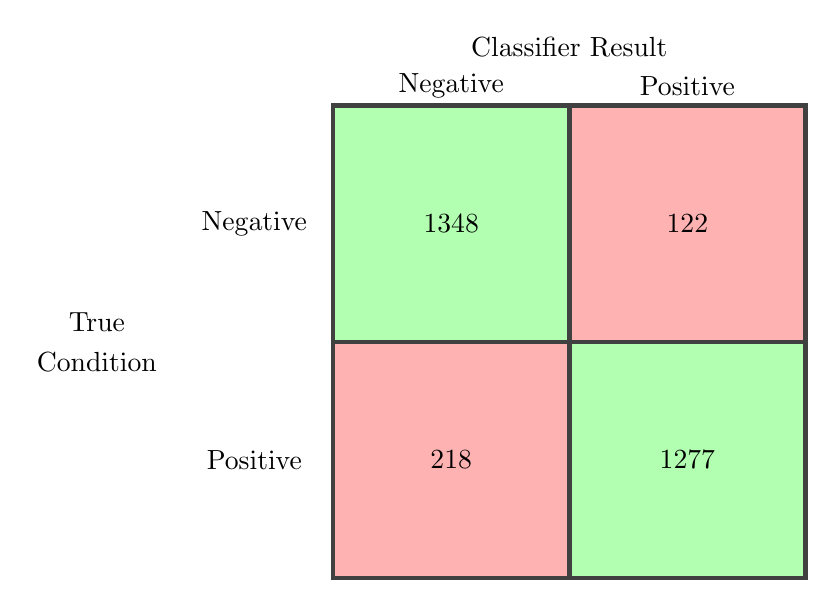
\begin{tikzpicture}[ultra thick]
        \filldraw[fill=green!30,draw=gray!50!black] (-3,3) rectangle (0,0);
        \filldraw[fill=red!30,draw=gray!50!black] (3,3) rectangle (0,0);
        \filldraw[fill=red!30,draw=gray!50!black] (-3,-3) rectangle (0,0);
        \filldraw[fill=green!30,draw=gray!50!black] (3,-3) rectangle (0,0);
        \node[] at (-6,0.25) {True};
        \node[] at (-6,-0.25) {Condition};
        \node[] at (-4,-1.50) {Positive};
        \node[] at (-4,1.50) {Negative};
        \node[] at (-0,3.75) {Classifier Result};
        \node[] at (-1.5,3.25) {Negative};
        \node[] at (1.5,3.25) {Positive};
        \node[] at (-1.5,1.5) {1348};
        \node[] at (1.5,1.5) {122};
        \node[] at (-1.5,-1.5) {218};
        \node[] at (1.5,-1.5) {1277};
    \end{tikzpicture}
    \label{fig:confusion}
    \caption{Confusion Matrix For Classifier: Total Cases: 2965, True Negatives:
    1348, False Positives: 122, False Negatives: 218, True Positives: 1277}
\end{figure}

\section{Conclusion}
The beat classification algorithm performed surprisingly well given its
simplicity and how the data are clustered in Figure \ref{fig:classifier}.  The
sensitivity and specificity are reasonably high but could definitely be improved
with more-sophisticated classification techniques, such as a support vector
machine or artificial neural network.  This algorithm is not particularly
remarkable, but is an excellent starting point for future development.  

In retrospect, picking an arrhythmia that is very similar to a normal rhythm on
an ECG made classification significantly harder.  If an arrhythmia presenting a
more-drastic difference on the ECG was chosen, the classifier would have likely
performed better.  An arrhythmia that is too different, though, would have made
QRS detection harder, since the algorithm is based on assumptions about what the
ECG will look like.  There is a trade-off between classifier performance and
QRS-detection performance.  

\newpage
\appendix
\section{Matlab Code}
\subsection{\texttt{fetch()}}
\label{fun:fetch}
\lstinputlisting{../matlab/fetch.m}

\subsection{\texttt{filterecg()}}
\label{fun:filter}
\lstinputlisting{../matlab/filterecg.m}

\subsection{\texttt{findqrs()}}
\label{fun:qrs}
\lstinputlisting{../matlab/findqrs.m}

\subsection{\texttt{crop()}}
\label{fun:crop}
\lstinputlisting{../matlab/crop.m}

\subsection{\texttt{pca\_transform()}}
\label{fun:pca}
\lstinputlisting{../matlab/pca_transform.m}

\subsection{\texttt{plotpca()}}
\label{fun:plotpca}
\lstinputlisting{../matlab/plotpca.m}

\subsection{\texttt{plotecg()}}
\label{fun:plotecg}
\lstinputlisting{../matlab/plotecg.m}

\subsection{\texttt{texify()}}
\label{fun:tex}
\lstinputlisting{../matlab/texify.m}

\subsection{\texttt{gather.m}}
\label{scr:gather}
\lstinputlisting{../matlab/gather.m}

\subsection{\texttt{train.m}}
\label{scr:train}
\lstinputlisting{../matlab/train.m}

\subsection{\texttt{figures.m}}
\label{scr:figures}
\lstinputlisting{../matlab/figures.m}

\bibliography{sources}
\bibliographystyle{IEEEtran}

\end{document}
